

% Section: DESIGN
\section{System Model and Design}
\label{sec:design}

Our incentive mechanism for community cloud targets real community networks so it must be integrated into an architecture, design and implementation which fits into these conditions and scenarios.
In this section, we first analyse the topology of community networks from which we develop two main cloud scenarios we foresee for them.
We then present the conceptual overview of a cloud management system suitable for community networks, of which we identify the resource assignment and regulation mechanism as a key component.



%%%%%%%%%%%%%%%%%%%%%%%%%%%%%%%%%%%%%%%%%%%%
\subsection{Topology of Community Networks}

The community network generally has two different types of nodes,  super nodes (SN) and ordinary nodes (ON). 
Super nodes have at least two wireless links, each to other super nodes.  
Most super nodes are installed in the community network participant's premises. 
A few super nodes, however are placed strategically on third party location, e.g. telecommunication installations of municipalities, to improve the community network's backbone.
Ordinary nodes only connect to a super node, but do not route any traffic. 
A topological analysis of the Guifi.net community network~\cite{Vega2012} indicates that from approximately 17,000 analysed nodes of Guifi.net, 7\% are super nodes while the others are ordinary nodes.



%%%%%%%%%%%%%%%%%%%%%%%%%%%%%%%%%%%%%%%%%%%%
\subsection{Community Cloud Scenarios}

The scenario of \emph{local community cloud} is derived from the topology of community network and the observed characteristics of the strength of the social network within community network zones. 
In the local community cloud, a super node is responsible for the management of a set of attached nodes contributing cloud resources. 
From the perspective of the attached nodes, this super node acts as a centralised unit to manage the cloud services. 

Multiple super nodes in a community network can connect and form \emph{federated community clouds}~\cite{Moreno-Vozmediano2012}.
The super node connects physically with other super nodes through wireless links and logically in an overlay network to other SNs that manage local clouds.
SNs coordinate among each other and the requests originating from one SN's zone can therefore be satisfied by the resources allocated from another SN's zone.



%%%%%%%%%%%%%%%%%%%%%%%%%%%%%%%%%%%%%%%%%%%%
\subsection{Community Cloud Manager}
\label{sec:arch-cloud-manager}

The option we foresee for enabling a cloud in a community network is deploying a cloud management system tailored to community networks on a super node. 
We propose a conceptual overview for such a system in Figure~\ref{fig:overview-vmm-hierarchy} which consists of the following.

\begin{itemize}
    \item The ordinary nodes of the community network provide hardware resources isolated as virtual machine (VM) instances and form the hardware layer of the cloud architecture. 
    \item The core layer residing in the super node contains the software for managing the virtual machines on ordinary nodes.
    \item The cloud coordinator is responsible for the federation of the cloud resources which are independently managed by different local community clouds.
        The cloud coordinator components in different SNs connect with each other in a decentralised manner to exchange relevant information about managing the available resources.
    \item The front end layer provides the interface for accessing resources from the cloud as Infrastructure-as-a-Service (IaaS).
\end{itemize}
    

The core of cloud management system is virtual machine manager that is responsible for instantiating, scheduling and monitoring virtual machines on the nodes.
There are some cloud management systems available to manage public and private clouds, for example OpenNebula~\cite{Moreno-Vozmediano2012} and OpenStack~\cite{Openstack} are among the most consolidated and popular open source tools.
Such cloud management systems are then tailored for community networks by extending them with implementing the cloud coordinator and its services on top of them, to address the particular conditions of community networks.

%% Figure 
\begin{figure}[htb]
   \centering
   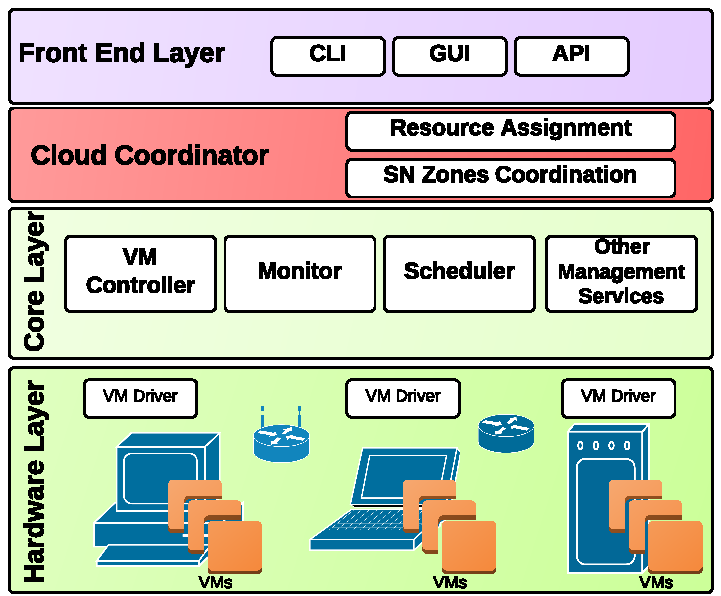
\includegraphics[width=3.5in,keepaspectratio]{vmm-architecture-generic}
   \caption{Conceptual overview of the Community Cloud Manager}
   \label{fig:overview-vmm-hierarchy}
\end{figure}


%%%%%%%%%%%%%%%%%%%%%%%%%%%%%%%%%%%%%%%%%%%%
\subsection{Incentive Mechanisms in Community Cloud}
\label{sec:incentives-architecture}

Participants in a community network are mainly volunteers that act independently and are not obliged to contribute. 
To ensure sustainability and growth of the community cloud, incentive mechanisms are needed that encourage members to contribute with their hardware, effort and time~\cite{Biczok2011, Bina2006}.
When designing such mechanisms, the heterogeneity of the nodes and communication links has to be considered since each member brings in a widely varying set of resources and physical capacity to the system.

Most peer-to-peer (P2P) systems implement incentive mechanisms based on contribution where nodes are rewarded according to resources they donate to the system~\cite{Zhang2010}.
We suggest an effort-based incentive mechanism for community cloud where effort is defined as contribution relative to the capacity of a node~\cite{Buyksahin2013}. 
This mechanism is inspired by the \emph{Parecon} economic model~\cite{Rahman2010, Vega2013Effort, Vega2013Sharing} which focuses on social welfare by considering inequality among nodes. 
Nodes with different capacity cannot have same contribution to the system but in this mechanism they get same reward if they share as much as possible of their capacity as we explain in the following.


%%%%%%%%%%%%%%%%%%%%%%%%%%%%%%%%%%%%%%%%%%%%
\subsubsection{Formulations}
% Calculation of Transaction Cost and Credits

We first discuss here the criteria that a super node uses to evaluate requests from ordinary nodes.
When a node asks for a resource from a SN, which in this case means to commit an instance of virtual machine for a given duration, the SN first checks whether the ON's credit is sufficient to cover the cost of the transaction.
The cost is proportional to the number of resources requested ${ R }_{ i }$ and the duration ${ T }_{ i }$ for how long they are required.

\begin{equation}
transaction\_cost = \gamma { R }_{ i } \times \rho { T }_{ i }
\end{equation}
where $\gamma$ and $\rho$ are nonzero coefficients for the amount and duration of resources shared respectively.

If the requesting node does not have enough credit, the request is rejected. 
Otherwise, the SN searches for nodes that have resources available. 
It selects as many nodes as possible from its local zone as providers.
If the demand cannot be met locally, the SN forwards the request to super nodes in the federated community cloud.

Now we consider how the SN manages the credits of the nodes that take part in the transaction.
For each node which contributed its resources to fulfil the request, the SN calculates the transaction cost as shown above and adds it to that node's credits. 
The cost is deducted from the credits of the node that consumed the resources.
After the transaction is completed, the effort for each node involved in the transaction is recalculated as in \cite{Buyksahin2013} by:

\begin{equation}
    \begin{IEEEeqnarraybox}{rCl} % Note the equation uses IEEEeqnarray, so need to include \usepackage{IEEEtrantools}
        { E }_{ i }\quad = 
        \begin{cases}
            \frac{{credit}_{i}}{ \epsilon {C}_{i}} \quad if \quad \frac{{credit}_{i}}{ \epsilon {C}_{i}} < 1 \quad \\
            \quad 1  \qquad otherwise
        \end{cases}    
    \end{IEEEeqnarraybox}
\end{equation}

where $\epsilon$ is nonzero coefficient for the capacity of the node.
The effort of a node expresses its relative contribution to the system, since the mechanism considers the capacity ${ C }_{ i }$ of a node as well. 
This means that a node with low capacity puts in more effort than a node with high capacity if they both donate same amount of resources to the system.

The total amount of resources available ${\Omega}$ in the system is sum of the resources ${ { \omega } }_{ i }$ shared by each node.

\begin{equation}
    \Omega =  \sum _{ i }^{ all \quad nodes }{ { \omega  }_{ i } }  
\end{equation}

And the maximum resource ${ { \Delta R } }_{ i }$ a node can consume depends on its effort. 

\begin{equation}
    { \Delta R }_{ i } ={ E }_{ i } \times ( \Omega - { \omega  }_{ i })  
\end{equation}


%%%%%%%%%%%%%%%%%%%%%%%%%%%%%%%%%%%%%%%%%%%%
\subsubsection{Algorithm for Requests Processing}


%% ALGORITHM
\begin{figure}[bht!]
    \begin{algorithmic}[1]
        \REQUIRE{receive query from node \emph{i} with the requested amount ${ R }_{ i }$ and the time ${ T }_{ i }$ }
        \STATE calculate($\Delta { R }_{ i }$)
        \IF{${ { R }_{ i } <= \Delta R }_{ i } $}
            \STATE call Decision(\emph{i}, ${ R }_{ i }$, ${ T }_{ i }$)
        \ELSE
            \STATE send(``rejected'', \emph{i})
        \ENDIF
        \STATE \textbf{function} DECISION(${i}$, ${ R }_{ i }$, ${ T }_{ i }$)
        %\Procedure{Decision}{${i}$, ${ R }_{ i }$}
            \IF{${R}_{ i } <= \Omega$}
                \STATE  \emph{ProvidersList}[n]  $\leftarrow$ high\_score\_first(\emph{ON\_List}, ${ R }_{ i }$)
                \FOR{\textbf{each} j in \emph{ProviderList}[n]}
                    \STATE ${CostOfTransaction}_{j \rightarrow i} \leftarrow {R}_{ j }^{ r} * {T }_{ j }^{t}$
                \STATE update\_credits(${CostOfTransaction}_{j \rightarrow i}$) 
                \STATE update\_database($ON\_List$)
                \ENDFOR
            \ELSE
                \STATE \emph{SN} $\leftarrow$ low\_credit\_first(\emph{SN\_List},${ R }_{ i }, reserved\_ratio$)
                \STATE forward(\emph{SN},\emph{i}, ${ R }_{ i }, { T }_{ i }$ )
            \ENDIF
    %  \EndProcedure
    \end{algorithmic}
    \caption{Algorithm for handling requests from ordinary nodes}
    \label{fig:algo}
\end{figure}
%%%%%%%%%%%%%%%%%%%%%%

Figure~\ref{fig:algo} shows algorithm for how a SN handles request from a node in its zone.
When SN receives request, it first calculates that node's allowance $\Delta {R }_{ i }$ to confirm whether it has enough credit to fulfil the request. 
If not, the request is rejected, otherwise the algorithm calls \emph{decision} function which searches for available resources (lines 1--5).
 
The \emph{decision} function first checks if enough resources are available in the local zone (line 8), and selects the nodes that will provide the resources from its local zone using \emph{high-score-first} policy (line 9).
The idea is to give preference to the nodes that need credit the most for participating in the system.
If SN cannot satisfy request from its local nodes, it forwards request to one of its neighbouring super nodes which is chosen using \emph{low-credit-first} policy (lines 16--18).
This allows the zone with depleted credits to earn more so its nodes can be active the system again. 
After the provider nodes commit resources, SN calculates cost of the transaction and updates the 
nodes' credits, deducting credits from the requester and increasing credits of the providers (lines 10--14).


%%%%%%%%%%%%%%%%%%%%%%%%%%%%%%%%%%%%%%%%%%%%
\subsubsection{Policies for Nodes Selection}
When SN processes requests for resources, there may be multiple nodes that can be providers so SN applies a selection policy for prioritising which nodes to choose.
Similarly when SN forwards requests to other SN zones, it also has to select between multiple zones that have resources available.
We evaluated a number of selection criteria that can be employed in above algorithm, and observed in experiments that \emph{low-credit-first} and \emph{high-score-first} policies were better in terms of efficiency of the system. 
In the following we explain these different policies and discuss the motivation behind them.

\begin{itemize}

\item \textbf{Low Credit First Selection.}
When nodes consume resources, their credit gets spent and with time their credit may be too low to request any resources.
Such nodes can provide their resources to other nodes and earn credit allowing them to participate in the system again.
This policy gives priority to nodes with low credit with the aim to ensure that most nodes participate in the system and are not left out because of lack of credit.

When multiple SN zones participate in the system, same problem exists since nodes in a particular zone may have all spent their credit and cannot request any more resources.
So the algorithm above gives preference to such zones by applying low-credit-first policy when selecting other SNs to forward requests.

\item \textbf{High Score First Selection.}
One issue with the low-credit-first approach is that it does not differentiate among nodes with low credit. 
Some of the nodes may be inactive and not making any requests while others may be getting their requests rejected because of inadequate credit. 
In this policy, the SN tracks unsuccessful attempts by each node and assigns it a \emph{score} calculated as follows. Nodes with higher score get preference so they can recover their credit.

\begin{equation}
    {score}_{ i } =   \frac{{attempts}_{ i }}{{credit}_{ i }}  
\end{equation}

\item \textbf{Other Policies.}
We also considered following policies and compared their effect on efficiency of the system.

    \begin{itemize}
        \item First-in-first-out (FIFO). In this simple policy, as soon as nodes have free resources, they register their availability with SN which keeps on adding them in a queue. When processing requests, the SN selects a node that has been in the queue the longest.
        
        \item Random. In this policy, SN picks a node at random from the queue.
        
        \item High credit first. This is the opposite of low-credit-first policy and here nodes with more credits are chosen first.
    \end{itemize}

\end{itemize}

